\documentclass[11pt]{article}
\usepackage{notes}
\definecolor{AccN}{HTML}{0D5C6F}
\begin{document}
\titlepg{4}{Unsupervised Learning Part 1:\\Clustering and Dimensionality Reduction}{$k$-Means, DBSCAN, Gaussian mixtures and EM, hierarchical clustering, PCA, t-SNE and UMAP --- discovering OPFOR archetypes without labels}
\tableofcontents
\newpage

\section{Why Unsupervised Learning?}
Supervised learning needs a label for every example, and labels can only name categories that analysts already know. Clustering asks instead: ``What natural groupings exist in these 8,000 trajectories?'' It can reveal tactics that no analyst has yet thought to label --- the defining strength of unsupervised learning in intelligence work.
\begin{definition}{clustering}
Partitioning unlabelled data $\{x_i\}$ into groups (clusters) such that points within a cluster are more similar to each other than to points in other clusters. Families: partitional ($k$-Means, GMM), density-based (DBSCAN), hierarchical (agglomerative), plus dimensionality reduction (PCA, t-SNE, UMAP) for compression and visualisation.
\end{definition}
\textbf{Case study.} $N=8{,}000$ OPFOR force-movement trajectories from JANUS exercise logs (10 armies $\times$ 800), with 12 features: average and maximum speed, direction-change rate, formation spread, dwell time, terrain exposure, route deviation, engagement frequency, time-of-day, weather, mission phase and force-size category. All features are z-scored, because distance-based clustering is meaningless when one feature ranges 0--200 and another 0--1.

\section{$k$-Means}
\subsection{Objective and Lloyd's algorithm}
\[J=\sum_{j=1}^k\sum_{x_i\in C_j}\|x_i-\mu_j\|^2\quad\text{(within-cluster sum of squares, WCSS).}\]
Lloyd's algorithm alternates: \textbf{assign} each point to its nearest centroid, $c_i=\arg\min_j\|x_i-\mu_j\|^2$; \textbf{update} each centroid to the mean of its points, $\mu_j=\frac1{|C_j|}\sum_{x_i\in C_j}x_i$.
\begin{derivation}{why the algorithm converges}
The assignment step cannot increase $J$ (each point moves to a closer centroid), and the update step cannot increase $J$ (the mean minimises the sum of squared distances to a set of points: setting $\partial/\partial\mu\sum\|x_i-\mu\|^2=-2\sum(x_i-\mu)=0$ gives the mean). $J$ is bounded below by zero and there are finitely many partitions, so the algorithm terminates --- at a \emph{local} minimum, not necessarily the global one.
\end{derivation}
Remedies for poor local minima: $k$-means++ initialisation (choose each new centre with probability proportional to its squared distance from existing centres; about 16 times better WCSS in practice) and multiple restarts (10 or more), keeping the lowest $J$. Cost is $O(Nkd)$ per iteration: $8000\times5\times12=480{,}000$ operations, under half a second in total.

\subsection{Assumptions}
$k$-Means assumes roughly spherical, similarly sized clusters of similar density, measured with Euclidean distance on comparable scales. It fails on rings and elongated shapes, on clusters of very different density, and in the presence of noise, and it cannot choose $k$.

\subsection{Choosing $k$}
WCSS always falls as $k$ grows (it is zero when $k=N$), so look for the \emph{elbow} where further clusters buy little: here WCSS drops 42,240 from $k=1$ to 2, 17,570 to 3, 9,680 to 4, 6,490 to 5, then only 3,180, 1,720, 720, 540, 300.
\begin{definition}{silhouette}
For point $i$, let $a(i)$ be its mean distance to points in its own cluster and $b(i)$ the mean distance to points in the nearest other cluster. Then $s(i)=\frac{b(i)-a(i)}{\max\{a(i),b(i)\}}\in[-1,1]$. Values near 1 mean well clustered, near 0 on a boundary, negative probably misassigned. The mean silhouette $S>0.7$ indicates strong structure; $<0.25$ weak structure.
\end{definition}
Silhouette was 0.481, 0.534, 0.638, \textbf{0.712}, 0.664, 0.601 for $k=2$--7, confirming $k=5$.
\begin{center}\begin{tikzpicture}\begin{axis}[width=9cm,height=4.5cm,xlabel={$k$},ylabel={WCSS},xmin=0.6,xmax=10.4,ymin=0,ymax=100000,xtick={1,...,10},grid=major,scaled y ticks=false,yticklabel style={/pgf/number format/fixed}]
\addplot[AccN,thick,mark=*]coordinates{(1,94420)(2,52180)(3,34610)(4,24930)(5,18440)(6,15260)(7,13540)(8,12820)(9,12280)(10,11980)};\draw[RedN,thick](axis cs:5,18440)circle(0.2cm);
\end{axis}\end{tikzpicture}\\*{\small\color{GreyN}Figure 1: the elbow at $k=5$.}\end{center}

\subsection{The five archetypes}
\begin{center}\small\renewcommand{\arraystretch}{1.2}
\begin{tabular}{lrrrrrl}\toprule Cluster & Size & Avg spd & Dir chg & Spread & Dwell & Archetype\\\midrule C-0 & 1,542 & 18.3 & 3.2 & 420 m & 22.4 min & patrol\\ C-1 & 932 & 62.7 & 28.4 & 85 m & 1.8 min & assault\\ C-2 & 714 & 41.2 & 6.1 & 310 m & 4.2 min & transit\\ C-3 & 2,184 & 4.8 & 1.2 & 380 m & 61.2 min & static/defensive\\ C-4 & 628 & 29.4 & 18.7 & 140 m & 8.6 min & \textbf{infiltration}\\\bottomrule\end{tabular}\end{center}
Cluster C-4 --- moderate speed, tight formation, evasive direction changes, mostly at night --- was not in the analysts' label scheme. It was named only after experts examined its members: \textbf{an enemy tactic discovered without labels}. Agreement with 200 expert-labelled trajectories was 87.0\% overall (94.6\% for static, 76.4\% for the new infiltration class).
\begin{pitfall}{internal consistency}
The listed cluster sizes sum to 6,000 rather than 8,000, and the GMM mixture weights reported later sum to 0.75 rather than 1. They appear to describe a 6,000-trajectory subset. Always check that reported partitions account for the whole dataset.
\end{pitfall}

\section{DBSCAN: Density-Based Clustering}
\begin{definition}{core, border and noise points}
With radius $\varepsilon$ and threshold MinPts: a \textbf{core point} has at least MinPts points within distance $\varepsilon$; a \textbf{border point} lies within $\varepsilon$ of a core point but is not itself core; a \textbf{noise point} is neither. Clusters are maximal sets of density-connected points (reachable through chains of core points).
\end{definition}
DBSCAN finds clusters of arbitrary shape, discovers their number automatically, and labels outliers explicitly rather than forcing them into a cluster. With a spatial index it runs in $O(N\log N)$.

\textbf{Choosing parameters.} Plot each point's distance to its MinPts-th nearest neighbour in sorted order and place $\varepsilon$ at the knee ($\varepsilon=0.45$ here). MinPts controls how much is called noise: 5 gave 42 noise points (0.5\%), 8 gave 142 (1.8\%), 15 gave 318 (4.0\%); a common rule is MinPts $\ge d+1$.

\textbf{Case-study result.} DBSCAN found four clusters --- merging patrol and static into one dense group --- plus \textbf{142 noise trajectories}: night operations (89\%), small single units (82\%), near-zero dwell, direction change 34.2 deg/min and route deviations above 820 m. Experts identified them as \textbf{deliberate deception manoeuvres}; $k$-Means would have hidden each one inside its nearest archetype. Limitation: one $\varepsilon$ cannot suit clusters of very different density; HDBSCAN extracts stable clusters across density scales.

\section{Gaussian Mixture Models and EM}
\[P(x)=\sum_{k=1}^K\pi_k\,\mathcal N(x;\mu_k,\Sigma_k),\qquad\sum_k\pi_k=1.\]
Each cluster is a Gaussian with its own mean and full covariance, allowing elliptical clusters of different sizes and orientations. Membership is soft: the \textbf{responsibility}
\[r_{ik}=\frac{\pi_k\mathcal N(x_i;\mu_k,\Sigma_k)}{\sum_j\pi_j\mathcal N(x_i;\mu_j,\Sigma_j)}\]
is the probability that point $i$ came from component $k$. Trajectory $T_{481}$ had $r(\text{assault})=0.62$ and $r(\text{infiltration})=0.38$, so it can be flagged as ambiguous instead of silently labelled. $k$-Means is the limiting case of a GMM with equal spherical covariances shrinking to zero.

\subsection{The EM algorithm}
Maximising $\mathcal L(\theta)=\sum_i\log\sum_k\pi_k\mathcal N(x_i;\mu_k,\Sigma_k)$ directly is hard because of the log of a sum. EM alternates:
\begin{itemize}
\item \textbf{E-step:} compute $r_{ik}$ with the current parameters.
\item \textbf{M-step:} $N_k=\sum_ir_{ik}$, $\pi_k=N_k/N$, $\mu_k=\frac1{N_k}\sum_ir_{ik}x_i$, $\Sigma_k=\frac1{N_k}\sum_ir_{ik}(x_i-\mu_k)(x_i-\mu_k)^\top$.
\end{itemize}
Each iteration never decreases the likelihood. In the case study, initialised from $k$-Means, log-likelihood rose from $-38{,}214$ to $-24{,}519$ in 65 iterations. Pitfalls: local maxima (use several starts), singular covariances when a component collapses onto one point (add $\varepsilon I$), and label switching between runs. \textbf{Model selection} uses $\text{AIC}=2p-2\log L$ or $\text{BIC}=p\log N-2\log L$; both were minimised at $K=5$, while raw likelihood kept increasing with $K$.

\section{Hierarchical Clustering}
Agglomerative clustering starts with every point as its own cluster and repeatedly merges the two closest clusters, producing a tree (dendrogram). Linkage defines ``closest'': single (nearest pair; produces chains), complete (farthest pair; compact clusters), average, or \textbf{Ward} (the merge that least increases WCSS; compact clusters, preferred here). Cutting the dendrogram at the largest vertical gap gives the number of clusters. Memory and time are $O(N^2)$ --- 8 s for 8,000 points, impractical for millions.

In the case study (2,000-trajectory subsample) assault and infiltration merged at height 0.83, the closest pair; cutting at 1.5 gave five clusters. The \textbf{adjusted Rand index} between Ward and $k$-Means partitions was 0.847 (1 = identical, 0 = chance), so two very different methods agreed --- strong evidence that the five archetypes are real. The dendrogram itself is a useful intelligence product, showing which behaviours are most alike.

\section{Principal Component Analysis}
\begin{derivation}{PCA as eigen-decomposition}
Centre the data, $\bar X=X-\text{mean}$, and form the covariance $C=\frac1N\bar X^\top\bar X$. The direction $v$ (unit length) that maximises the projected variance $v^\top Cv$ satisfies, by a Lagrange multiplier, $Cv=\lambda v$: it is the leading eigenvector, and the variance along it equals the eigenvalue $\lambda$. Successive components are the remaining eigenvectors, mutually orthogonal. Projecting onto the top $k$ gives scores $Z=\bar XV_k$; the explained-variance ratio of component $j$ is $\lambda_j/\sum_i\lambda_i$. Numerically, use the SVD $\bar X=USV^\top$ with $\lambda_j=s_j^2/(N-1)$.
\end{derivation}
\begin{center}\begin{tikzpicture}[x=0.8cm,y=0.8cm]
\foreach \x/\y in {-2.2/-1.1,-1.8/-0.6,-1.4/-0.9,-1.0/-0.2,-0.6/-0.5,-0.2/0.1,0.2/-0.1,0.6/0.4,1.0/0.2,1.4/0.8,1.8/0.6,2.2/1.2,-1.6/-1.2,0.9/0.7,-0.3/-0.4,1.6/1.1}{\fill[BluN](\x,\y)circle(0.06);}
\draw[-{Stealth},AccN,line width=1.5pt](0,0)--(2.4,1.25)node[right,font=\small]{PC1};\draw[-{Stealth},RedN,line width=1.3pt](0,0)--(-0.45,0.85)node[above,font=\small]{PC2};
\end{tikzpicture}\\*{\small\color{GreyN}Figure 2: principal components align with the directions of greatest spread.}\end{center}
Case study eigenvalues: 4.21, 2.84, 1.62, 1.45, 0.72, \ldots; the first four components explain 84.4\% of variance (Kaiser rule $\lambda>1$), six explain over 95\%. Loadings give meaning: PC1 (speed 0.48, maximum speed 0.41, direction change 0.38) is an ``activity/aggression'' axis; PC2 (spread 0.52, dwell 0.44, exposure 0.31) a ``dispersion/caution'' axis.

\section{t-SNE and UMAP}
PCA is linear and cannot unfold curved manifolds. \textbf{t-SNE} converts high-dimensional distances into neighbour probabilities $p_{ij}$ (Gaussian kernels whose widths are set by the \emph{perplexity}, typically 5--50) and finds 2-D points whose Student-$t$ neighbour probabilities $q_{ij}$ match, by minimising $\sum p_{ij}\log(p_{ij}/q_{ij})$. It preserves local neighbourhoods; \textbf{distances between clusters and cluster sizes in a t-SNE plot are not meaningful}. \textbf{UMAP} builds a neighbourhood graph and optimises a similar layout; it was 9 times faster here (4.2 s vs 38.4 s), preserves more global structure, is deterministic with a fixed seed, and can project new points into an existing map.

\section{Validating Clusters}
Use several measures: silhouette (0.712); Calinski--Harabasz (ratio of between- to within-cluster dispersion; 1,842, higher is better); Davies--Bouldin (average worst-case similarity of each cluster to another; 0.68, lower is better); Dunn index (smallest inter-cluster distance over largest intra-cluster diameter; 0.41); ARI against expert labels (0.870); bootstrap stability (re-cluster resampled data, average ARI 0.893). The \textbf{gap statistic} compares $\log$ WCSS with that expected for structureless reference data and also peaked at $k=5$; \textbf{prediction strength} (do pairs clustered together in one half stay together in the other?) was 0.887.

\section{Comparison and Workflow}
\begin{center}\small\renewcommand{\arraystretch}{1.2}
\begin{tabular}{lcccccc}\toprule Method & $k$ & Silhouette & ARI & Noise & Train & Strength\\\midrule $k$-Means & 5 (input) & 0.712 & 0.870 & none & 0.8 s & fast, interpretable\\ DBSCAN & 4 (auto) & 0.684 & 0.821 & 142 & 2.1 s & any shape, flags noise\\ GMM & 5 (input) & 0.698 & 0.857 & none & 18.4 s & soft membership\\ Ward & 5 (cut) & 0.701 & 0.847 & none & 8.3 s & dendrogram\\\bottomrule\end{tabular}\end{center}
Recommended workflow: $k$-Means for a fast first pass $\to$ GMM initialised from it for probabilities $\to$ hierarchical clustering for visual confirmation $\to$ DBSCAN to surface noise and deception.

\section{Deeper Dive I: Distance, Scaling and Initialisation}
\subsection{Why scaling changes the clusters}
\begin{example}{speed vs exposure}
Two features: average speed (0--120 km/h) and terrain exposure (0--1). Trajectory A $(40,\,0.1)$, B $(42,\,0.9)$, C $(60,\,0.1)$. Unscaled, $d(A,B)=\sqrt{4+0.64}=2.15$ and $d(A,C)=20$: A groups with B although their exposure differs completely. After standardising (s.d.\ of speed 20, of exposure 0.3), $d(A,B)=\sqrt{0.01+7.1}=2.67$ and $d(A,C)=\sqrt{1+0}=1.0$: now A groups with C. The clustering --- and the tactical story --- depends entirely on scaling.
\end{example}
Standardisation treats every feature as equally important; if domain knowledge says otherwise, weight features explicitly after standardising.

\subsection{$k$-means++ seeding}
Choose the first centre uniformly at random; choose each subsequent centre with probability proportional to $D(x)^2$, its squared distance to the nearest centre already chosen. Points far from existing centres are likely to seed new clusters, which avoids two centres starting in the same group. The method carries a guarantee: expected WCSS within a factor $O(\log k)$ of optimal.
\begin{example}{seeding probabilities}
Points on a line at 0, 1, 10, 11 with first centre 0: squared distances 0, 1, 100, 121, total 222. The next centre is 10 with probability 0.45 and 11 with probability 0.55; only 0.5\% of the time is it 1 --- the bad choice.
\end{example}

\section{Deeper Dive II: Computing Validation Indices}
\subsection{Silhouette on a tiny dataset}
\begin{example}{full silhouette calculation}
Points 1, 2, 3 (cluster A) and 8, 9 (cluster B) on a line. For point 1: $a=(1+2)/2=1.5$, $b=(7+8)/2=7.5$, $s=6/7.5=0.80$. Point 2: $a=1$, $b=6.5$, $s=0.85$. Point 3: $a=1.5$, $b=5.5$, $s=0.73$. Point 8: $a=1$, $b=(7+6+5)/3=6$, $s=0.83$. Point 9: $a=1$, $b=7$, $s=0.86$. Mean silhouette $S=0.81$: strong structure.
\end{example}

\subsection{Calinski--Harabasz and Davies--Bouldin}
\[\text{CH}=\frac{\text{tr}(B_k)/(k-1)}{\text{tr}(W_k)/(N-k)},\qquad\text{DB}=\frac1k\sum_{i=1}^k\max_{j\ne i}\frac{s_i+s_j}{d(\mu_i,\mu_j)},\]
where $B_k$ and $W_k$ are the between- and within-cluster scatter matrices, $s_i$ the average distance of cluster $i$'s points to its centroid and $d(\mu_i,\mu_j)$ the distance between centroids. CH rewards well-separated, compact clusters (higher is better); DB measures each cluster's worst-case similarity to another (lower is better).

\subsection{The adjusted Rand index}
For two partitions of $N$ points, the Rand index is the fraction of the $\binom N2$ pairs on which they agree (both together or both apart). Random partitions agree on many pairs by chance, so the ARI subtracts the expected agreement: $\text{ARI}=\frac{\text{RI}-E[\text{RI}]}{\max\text{RI}-E[\text{RI}]}$, which is 0 for chance and 1 for identical partitions (it can be negative).
\begin{example}{a small ARI}
Partitions of four points: $P=\{\{1,2\},\{3,4\}\}$, $Q=\{\{1,2,3\},\{4\}\}$. Of the 6 pairs, both put (1,2) together and both separate (1,4) and (2,4): 3 agreements. Pairs (3,4), (1,3), (2,3) disagree. RI $=3/6=0.5$; after correction for chance the ARI here is 0, i.e.\ no better than random.
\end{example}

\section{Deeper Dive III: Gaussian Mixture Choices}
Covariance structure controls flexibility and parameter count. For $d$ features and $K$ components: \textbf{spherical} ($\sigma_k^2I$) has $K(d+1)$ mean-and-variance parameters; \textbf{diagonal} $2Kd$; \textbf{full} $K\big(d+d(d+1)/2\big)$; plus $K-1$ mixture weights. With $d=12$, $K=5$ full covariance needs $5(12+78)+4=454$ parameters --- which is why BIC's $p\log N$ penalty matters, and why diagonal covariances are used when data are scarce.
\begin{example}{BIC by hand}
Model 1: log-likelihood $-24{,}700$, $p=200$. Model 2: $-24{,}516$, $p=454$. With $N=8{,}000$, $\log N=8.99$. BIC$_1=200(8.99)+49{,}400=51{,}198$; BIC$_2=454(8.99)+49{,}032=53{,}113$. Despite its better fit, model 2 is penalised for 254 extra parameters, and BIC prefers model 1. (AIC, with penalty $2p$, gives $49{,}800$ vs $49{,}940$ and also prefers model 1, by a smaller margin.)
\end{example}

\section{Deeper Dive IV: Hierarchical Clustering in Action}
\begin{example}{agglomerative merging with single linkage}
Points 1, 2, 4, 7, 11 on a line. Distances between neighbours: 1, 2, 3, 4. Single linkage merges $\{1,2\}$ at height 1, then adds 4 at height 2, then 7 at height 3, then 11 at height 4. The dendrogram is a ``staircase'': single linkage chains points together. Ward linkage on the same data would instead merge $\{1,2\}$, then $\{1,2,4\}$, then $\{7,11\}$ (merge costs 4.2 and 8.0) and join the two groups last, giving two compact clusters.
\end{example}
\begin{center}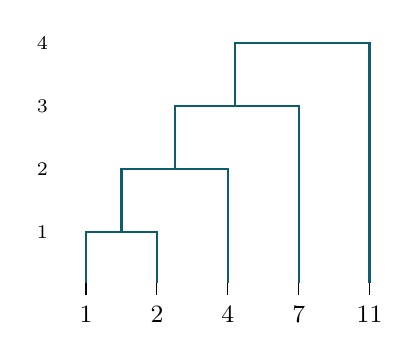
\begin{tikzpicture}[x=0.9cm,y=0.8cm]
\foreach \x/\l in {0/1,1/2,2/4,3/7,4/11}{\node[font=\small]at(\x,-0.3){\l};\draw(\x,0)--(\x,0.2);}
\draw[thick,AccN](0,0.2)--(0,1)--(1,1)--(1,0.2);\draw[thick,AccN](0.5,1)--(0.5,2)--(2,2)--(2,0.2);\draw[thick,AccN](1.25,2)--(1.25,3)--(3,3)--(3,0.2);\draw[thick,AccN](2.1,3)--(2.1,4)--(4,4)--(4,0.2);
\foreach \h in {1,2,3,4}{\node[font=\scriptsize,anchor=east]at(-0.4,\h){\h};}
\end{tikzpicture}\\*{\small\color{GreyN}Figure 3: single-linkage dendrogram --- chaining.}\end{center}

\section{Deeper Dive V: PCA from Raw Data}
\begin{example}{PCA on four trajectories}
Centred data (speed, direction change): $(-2,-1)$, $(-1,-1)$, $(1,1)$, $(2,1)$. Covariance (dividing by $N=4$): $\text{var}_1=(4+1+1+4)/4=2.5$, $\text{var}_2=1$, $\text{cov}=(2+1+1+2)/4=1.5$. Eigenvalues of $\begin{pmatrix}2.5&1.5\\1.5&1\end{pmatrix}$: $\lambda=\frac{3.5\pm\sqrt{(1.5)^2+4(2.25)}}{2}=\frac{3.5\pm3.354}{2}=3.43,\ 0.07$. PC1 explains 98\% of variance, direction $\propto(1.5,\,0.93)$, normalised $(0.85,0.53)$: speed and direction change rise together. Projecting onto PC1 reduces two features to one score with almost no loss; the reconstruction error equals the discarded eigenvalue (0.07 per point on average).
\end{example}
\begin{center}\begin{tikzpicture}\begin{axis}[width=8cm,height=4.3cm,xlabel={component},ylabel={eigenvalue},ybar,bar width=10pt,xtick={1,...,8},ymin=0,ymax=4.6,grid=major]
\addplot[fill=AccN!60]coordinates{(1,4.21)(2,2.84)(3,1.62)(4,1.45)(5,0.72)(6,0.44)(7,0.31)(8,0.20)};\draw[RedN,dashed](axis cs:0.5,1)--(axis cs:8.5,1);
\end{axis}\end{tikzpicture}\\*{\small\color{GreyN}Figure 4: case-study scree plot; dashed line is the Kaiser criterion $\lambda=1$.}\end{center}
\textbf{Scaling matters again:} PCA on unscaled data is dominated by the feature with the largest variance. Use the correlation matrix (i.e.\ standardise first) unless all features share units.

\section{Deeper Dive VI: Reading t-SNE and UMAP Responsibly}
Perplexity (roughly the effective number of neighbours) changes the picture: low values fragment data into many small islands; high values merge them. Run several perplexities and several random seeds; trust only structure that persists. UMAP's \texttt{n\_neighbors} plays a similar role, and \texttt{min\_dist} controls how tightly points pack. Neither method should be used to choose the number of clusters, and distances between islands are not interpretable.

\clearpage
\part*{Part C --- Further Theory, Methods and Applications}
\addcontentsline{toc}{part}{Part C --- Further Theory, Methods and Applications}

\section{Distance in High Dimensions}
\subsection{The curse of dimensionality}
Clustering assumes that ``near'' and ``far'' mean something. In high dimensions they stop doing so. Draw 500 points uniformly in a unit hypercube and measure their distances to a random query point; the relative contrast $(d_{\max}-d_{\min})/d_{\min}$ is about 29 in 2 dimensions, 2.5 in 10, 0.41 in 100 and 0.11 in 1,000. In 1,000 dimensions the nearest and farthest points are almost equally far away, so nearest-neighbour and centroid methods lose their footing.
\begin{center}\begin{tikzpicture}\begin{axis}[width=7cm,height=4.2cm,xmode=log,ymode=log,xlabel={dimension $d$},ylabel={$(d_{\max}-d_{\min})/d_{\min}$},grid=both,grid style={GreyN!20},font=\scriptsize]
\addplot[AccN,thick,mark=*]coordinates{(2,29.2)(10,2.54)(100,0.413)(1000,0.109)};
\end{axis}\end{tikzpicture}\\*{\small\color{GreyN}Figure C1: distance contrast collapses as dimension grows (500 uniform points).}\end{center}
Remedies: reduce dimension first (PCA, autoencoders), select informative features, use distances suited to the data (cosine for text, dynamic time warping for trajectories), and prefer methods that use local density or graph structure.
\subsection{What makes a distance}
A \textbf{metric} satisfies non-negativity, identity ($d(x,y)=0$ only if $x=y$), symmetry and the triangle inequality. Euclidean, Manhattan and Mahalanobis distances are metrics; cosine \emph{dissimilarity} $1-\cos\theta$ is not (it violates the triangle inequality), and neither is DTW --- which matters for algorithms that rely on the triangle inequality to prune computations.

\section{DBSCAN by Hand}
\begin{example}{one-dimensional DBSCAN}
Positions (km along a road) of ten detected vehicles: 1.0, 1.5, 2.0, 2.4, 5.0, 8.0, 8.6, 9.1, 9.5, 12.0. Parameters $\varepsilon=1.0$ km, MinPts $=3$ (counting the point itself).\\[2pt]
\textbf{Neighbour counts:} 1.0 has $\{1.0,1.5,2.0\}$: 3, core. 1.5: 4, core. 2.0: 4, core. 2.4: $\{1.5,2.0,2.4\}$: 3, core. 5.0: 1. 8.0: $\{8.0,8.6\}$: 2, not core. 8.6: 4, core. 9.1: 3, core. 9.5: 3, core. 12.0: 1.\\
\textbf{Clusters:} the core points 1.0--2.4 are mutually density-reachable: cluster~1. The core points 8.6--9.5 form cluster~2; 8.0 is not core but lies within $\varepsilon$ of the core point 8.6, so it is a \textbf{border} point of cluster~2. The points at 5.0 and 12.0 are \textbf{noise}.\\
\textbf{Reading it:} two convoy groups and two isolated vehicles. Whether the isolated vehicles are stragglers, scouts or decoys is a question for the analyst --- DBSCAN's contribution is to separate them rather than force them into a convoy as $k$-means would.
\end{example}
\begin{center}\begin{tikzpicture}[x=1.15cm,font=\scriptsize]
\draw[-{Stealth},GreyN](0.5,0)--(12.8,0);\foreach \t in {1,2,...,12}{\draw[GreyN](\t,0.08)--(\t,-0.08);\node[below,GreyN]at(\t,-0.1){\t};}
\foreach \p in {1.0,1.5,2.0,2.4}{\fill[BluN](\p,0.35)circle(3.2pt);}
\foreach \p in {8.6,9.1,9.5}{\fill[GrnN](\p,0.35)circle(3.2pt);}
\draw[GrnN,thick,fill=white](8.0,0.35)circle(3.2pt);
\foreach \p in {5.0,12.0}{\node[RedN,font=\small]at(\p,0.35){$\times$};}
\node[BluN]at(1.7,0.85){cluster 1 (core)};\node[GrnN]at(8.9,0.85){cluster 2};\node[GrnN]at(7.6,-0.6){8.0 = border};\node[RedN]at(5.0,0.85){noise};\node[RedN]at(12.0,0.85){noise};
\end{tikzpicture}\\*{\small\color{GreyN}Figure C2: DBSCAN result; filled = core, hollow = border, $\times$ = noise.}\end{center}

Variants: \textbf{OPTICS} orders points by reachability distance and reveals clusters at all density levels at once; \textbf{HDBSCAN} builds a hierarchy over $\varepsilon$ and extracts the most stable clusters, removing the need to choose $\varepsilon$ and handling clusters of different densities --- often the best default for exploratory work.

\section{The EM Algorithm Worked Through}
\begin{example}{three iterations of EM}
Six speeds: 1, 2, 3, 8, 9, 10. Two components, initialised badly: $\mu=(2,6)$, $\sigma=(2,2)$, $\pi=(0.5,0.5)$.\\[2pt]
\textbf{Iteration 1.} E-step responsibilities for component~1: $0.953,0.881,0.731,0.018,0.007,0.002$. M-step: $\mu=(1.98,\,8.18)$, $\sigma=(1.04,\,2.31)$, $\pi=(0.43,\,0.57)$. Log-likelihood $-17.19$.\\
\textbf{Iteration 2.} Responsibilities sharpen to $0.993,0.984,0.928,0,0,0$; $\mu=(1.98,8.80)$, $\sigma=(0.81,1.37)$. Log-likelihood $-13.57$.\\
\textbf{Iteration 3.} Responsibilities $1,1,1,0,0,0$; $\mu=(2,9)$, $\sigma=(0.82,0.82)$, $\pi=(0.5,0.5)$. Log-likelihood $-12.07$.\\[2pt]
The log-likelihood rises at every iteration, as EM guarantees, and the second component moves from its poor start at 6 to the true group at 9. Notice that component~1's point at 3 kept 7\% responsibility for component~2 after the first iteration: EM shares ambiguous points rather than assigning them outright.
\end{example}
\textbf{Why EM never decreases the likelihood.} The E-step builds a lower bound on the log-likelihood that touches it at the current parameters (by Jensen's inequality); the M-step maximises that bound. Climbing a bound that touches the function cannot take you downhill. Like $k$-means, EM finds a local maximum, so several starts are used; it can also collapse a component onto a single point (variance $\to0$, likelihood $\to\infty$), which software prevents with a small variance floor.
\subsection{Covariance choices}
\textbf{Spherical} (one variance per component), \textbf{diagonal} (independent features), \textbf{tied} (one shared full covariance) and \textbf{full} (each component its own ellipse). Parameters per component for $d$ features: 1, $d$, shared $d(d+1)/2$, and $d(d+1)/2$. With 12 features a full covariance needs 78 parameters per component; with limited data, simpler choices generalise better, and BIC arbitrates.

\section{Hierarchical Clustering in Depth}
\subsection{Linkage criteria}
The distance between two clusters $A$ and $B$ can be defined as:
\begin{itemize}
\item \textbf{single} --- the closest pair, $\min d(a,b)$: finds elongated shapes but suffers \emph{chaining}, linking distinct groups through a thin bridge of points;
\item \textbf{complete} --- the farthest pair, $\max d(a,b)$: compact clusters, sensitive to outliers;
\item \textbf{average} --- the mean of all pairwise distances: a compromise;
\item \textbf{Ward} --- the increase in total within-cluster sum of squares caused by merging, $\frac{|A||B|}{|A|+|B|}\|\mu_A-\mu_B\|^2$: compact, similar-sized clusters, consistent with $k$-means.
\end{itemize}
All four are updated efficiently after each merge by the Lance--Williams recurrence, so the full hierarchy for $N$ points costs $O(N^2)$ memory --- comfortable for thousands of trajectories, impractical for millions.
\subsection{Is the tree faithful?}
The \textbf{cophenetic distance} between two points is the height at which they first join in the dendrogram. Its correlation with the original pairwise distances (the cophenetic correlation) measures how faithfully the tree represents the data; values above about 0.8 indicate a good representation. Cutting the dendrogram at a height gives a flat clustering; a long vertical gap before a merge suggests a natural number of clusters.

\section{Spectral Clustering: Communities in a Graph}
Build a similarity graph with weights $W_{ij}$, degree matrix $D=\text{diag}(\sum_jW_{ij})$ and graph Laplacian $L=D-W$. For any vector $f$, $f^\top Lf=\frac12\sum_{ij}W_{ij}(f_i-f_j)^2$: small when strongly connected nodes have similar values. The eigenvectors of $L$ with the smallest eigenvalues are therefore smooth over the graph and change sign across weak links.
\begin{example}{two groups joined by a weak link}
Six radio nodes form two triangles $\{1,2,3\}$ and $\{4,5,6\}$ (edge weight 1), with one weak link of weight 0.1 between nodes 3 and 4. The Laplacian's eigenvalues are $0,\;0.064,\;3,\;3,\;3,\;3.136$. The second eigenvector (the \emph{Fiedler vector}) is $(0.42,0.42,0.39,-0.39,-0.42,-0.42)$: its sign splits the nodes into the two triangles, cutting only the weak link. The small second eigenvalue says the graph almost falls into two pieces.
\end{example}
\begin{center}\begin{tikzpicture}[font=\scriptsize,every node/.style={circle,draw=NavyN,minimum size=0.55cm,inner sep=0pt}]
\node[fill=BluN!15](1)at(0,0.9){1};\node[fill=BluN!15](2)at(0,-0.9){2};\node[fill=BluN!15](3)at(1.4,0){3};
\node[fill=AccN!20](4)at(3.4,0){4};\node[fill=AccN!20](5)at(4.8,0.9){5};\node[fill=AccN!20](6)at(4.8,-0.9){6};
\draw[thick](1)--(2);\draw[thick](1)--(3);\draw[thick](2)--(3);\draw[thick](4)--(5);\draw[thick](4)--(6);\draw[thick](5)--(6);
\draw[dashed,GreyN](3)--node[above,draw=none,font=\tiny]{0.1}(4);
\end{tikzpicture}\\*{\small\color{GreyN}Figure C3: the Fiedler vector's sign (blue positive, orange negative) cuts only the weak link.}\end{center}

Spectral clustering embeds the nodes using the first $k$ eigenvectors and runs $k$-means in that embedding. It finds non-convex clusters (rings, crescents) that defeat $k$-means, and it applies directly to network data --- communication graphs, social networks of interest --- where communities are what analysts want.

\section{Clustering Trajectories and Time Series}
Manoeuvre trajectories differ in speed and timing even when they follow the same pattern. Comparing them point by point (lock-step Euclidean distance) penalises a delay as heavily as a different route.
\subsection{Dynamic time warping}
DTW aligns two sequences by stretching time. With $C(i,j)=|a_i-b_j|+\min\{C(i-1,j),C(i,j-1),C(i-1,j-1)\}$ and $C(0,0)=0$, the DTW distance is $C(n,m)$.
\begin{example}{a delayed manoeuvre}
Range profiles of two approaches: $a=(0,1,2,3,2,0)$ and $b=(0,0,1,2,3,2,0)$ --- the same manoeuvre, one step later. Padding $a$ to equal length and comparing lock-step gives a distance of 6. DTW matches the extra 0 in $b$ to the first 0 of $a$ and then aligns the rest exactly: DTW distance 0. Clustering on DTW groups manoeuvres by shape rather than by timing.
\end{example}
DTW costs $O(nm)$ per pair; a band constraint (Sakoe--Chiba window) limits how far the alignment may stretch, which both speeds it up and prevents pathological matches. Alternatives are to summarise each trajectory by features (mean speed, heading-change rate, dwell time --- the approach of the Lecture~4 case study) or to learn embeddings with a sequence autoencoder.
\subsection{Other partitioning variants}
\textbf{$k$-medoids (PAM)} uses actual data points as cluster centres, works with any dissimilarity (including DTW) and resists outliers. \textbf{Mini-batch $k$-means} updates centroids from small random batches and scales to millions of points. \textbf{Kernel $k$-means} clusters in a kernel feature space and is closely related to spectral clustering.

\section{Dimensionality Reduction in Depth}
\subsection{PCA through the singular value decomposition}
For a centred data matrix $X$ ($N\times d$), the SVD $X=U\Sigma V^\top$ gives the principal directions as the columns of $V$ and the component variances as $\sigma_j^2/(N-1)$. Computing the SVD is numerically more stable than forming the covariance matrix and is how software actually performs PCA.
\subsection{How many components?}
Common rules: keep enough components to explain a target fraction of variance (80--95\%); look for the elbow in the \textbf{scree plot} of eigenvalues; or, for standardised data, keep components with eigenvalue above 1 (the \textbf{Kaiser rule} --- a component should explain more than one original feature's worth). In the Lecture~4 case, the eigenvalues 4.21, 2.84, 1.62, 1.45 all exceed 1 and together explain 84.4\% of the variance of 12 standardised features: both rules agree on four components.
\subsection{Reconstruction and whitening}
Projecting onto the first $q$ components and back gives the best rank-$q$ approximation of the data in squared error; the reconstruction error is the sum of the discarded eigenvalues. A point with large reconstruction error does not fit the main structure, which links PCA to anomaly detection (Lecture~5). \textbf{Whitening} divides each component by its standard deviation so that all have unit variance; it removes correlations and equalises scales before clustering.
\subsection{Beyond linear}
\textbf{Kernel PCA} performs PCA in a kernel feature space; \textbf{autoencoders} learn non-linear encodings with neural networks. \textbf{t-SNE} converts distances into neighbour probabilities --- Gaussian in the original space with a bandwidth set by the \emph{perplexity} (roughly the effective number of neighbours, typically 5--50), heavy-tailed Student-$t$ in the 2-D map --- and minimises the Kullback--Leibler divergence between them. Its heavy tails pull clusters apart, which is why t-SNE plots look so well separated and why the gaps between clusters, and their sizes, cannot be interpreted. \textbf{UMAP} builds a fuzzy neighbour graph and optimises a similar layout faster, preserving somewhat more global structure; the same caution applies.

\section{External Validation and Stability}
When some ground-truth labels exist (for a subset, or for a validation exercise), compare them with the clustering.
\begin{example}{purity, NMI and ARI}
Fourteen trajectories with known doctrine labels A (5), B (5), C (4) are clustered into three groups: cluster~0 contains A,A,A,A,B; cluster~1 contains B,B,B,B,A,C; cluster~2 contains C,C,C. \textbf{Purity} assigns each cluster its majority label and counts matches: $(4+4+3)/14=0.79$. \textbf{Normalised mutual information} is 0.50 and the \textbf{adjusted Rand index} 0.37. Purity flatters (it rises trivially as clusters are split); NMI and ARI correct for chance and are the measures to report.
\end{example}
\textbf{Stability.} Re-run the clustering on bootstrap resamples or sub-samples of the data and measure how consistently pairs of points end up together (for example, the mean ARI between runs). Real structure is stable; clusters that appear in some resamples and not others are probably artefacts of noise, initialisation or parameter choice.

\section{Clustering Text: Intelligence Reports}
Large volumes of reports, intercept transcripts and open-source articles are clustered to find themes.
\subsection{TF--IDF representation}
Each document becomes a vector with one entry per vocabulary word: the term frequency (share of the document's words) multiplied by the inverse document frequency $\ln(N/\text{df})$, which down-weights words that appear everywhere.
\begin{example}{TF--IDF for three short reports}
Reports: (1) ``armour bridge armour''; (2) ``bridge river engineer''; (3) ``armour artillery fire''. ``armour'' appears in 2 of 3 reports: idf $=\ln(3/2)=0.405$; in report~1 its tf is $2/3$, so tf--idf $=0.27$. ``bridge'' (tf $1/3$, idf 0.405) gives 0.135. ``river'' appears only in report~2 (idf $\ln3=1.10$), so where it occurs it is highly distinctive. Documents are then compared by cosine similarity and clustered.
\end{example}
\subsection{Topic models and embeddings}
\textbf{Latent Dirichlet allocation} models each document as a mixture of topics and each topic as a distribution over words, producing interpretable themes (``river crossing'', ``air defence''). Modern practice embeds documents with a pre-trained language model and clusters the embeddings (often with HDBSCAN), which captures meaning beyond shared words --- ``tank'' and ``armour'' land close together.
\begin{pitfall}{language and deception}
Text clusters reflect vocabulary and style as much as content: reports from different units, translations or deliberately misleading sources may cluster by author rather than by subject. Inspect representative documents from every cluster before naming it.
\end{pitfall}

\section{Further Self-Test Questions}
\begin{question}{Part C}
(1) In the DBSCAN example, what happens to the vehicle at 8.0 if MinPts is raised to 4? (2) Why can the EM log-likelihood never decrease? (3) What does a near-zero second Laplacian eigenvalue indicate? (4) Why is purity a poor measure on its own? (5) Two manoeuvres are identical except one starts 30 s later. Which distance treats them as the same?\\
\textit{Answers.} (1) Core points now need 4 neighbours: 1.5, 2.0 and 8.6 remain core (4 each); 1.0, 2.4, 9.1 and 9.5 become border points of their clusters; 8.0 is still within $\varepsilon$ of the core point 8.6, so it stays a border point. (2) Each iteration maximises a lower bound that equals the likelihood at the current parameters. (3) The graph nearly splits into two weakly connected communities. (4) It increases trivially with more clusters and ignores chance agreement. (5) Dynamic time warping.
\end{question}

\section{Implementation Notes}
\begin{center}\begin{minipage}{0.92\textwidth}\small\ttfamily
from sklearn.preprocessing import StandardScaler\\
from sklearn.cluster import KMeans, DBSCAN, AgglomerativeClustering\\
from sklearn.mixture import GaussianMixture\\
from sklearn.metrics import silhouette\_score, adjusted\_rand\_score\\[2pt]
Xs = StandardScaler().fit\_transform(X)\\
km = KMeans(n\_clusters=5, init="k-means++", n\_init=10, random\_state=0).fit(Xs)\\
db = DBSCAN(eps=0.45, min\_samples=8).fit(Xs) \quad \# labels\_ == -1 are noise\\
gm = GaussianMixture(5, covariance\_type="full", n\_init=5).fit(Xs) \quad \# gm.bic(Xs)\\
print(silhouette\_score(Xs, km.labels\_), adjusted\_rand\_score(km.labels\_, ward\_labels))
\end{minipage}\end{center}

\section{Self-Test Questions}
\begin{question}{five questions}
\textbf{1.} Why can the same data produce different clusters before and after standardisation? \textbf{2.} With centres at 0 and points at 0, 2, 6, what is the probability $k$-means++ picks 6 as the next centre? \textbf{3.} Why does BIC prefer simpler GMMs more strongly than AIC for large $N$? \textbf{4.} Which linkage tends to produce long chains, and why? \textbf{5.} A t-SNE plot shows two islands far apart. What may you conclude?

\textit{Answers.} 1: distances are dominated by large-scale features. 2: $36/(4+36)=0.9$. 3: its penalty $p\log N$ exceeds $2p$ once $N>e^2\approx7.4$ and grows with $N$. 4: single linkage --- merging depends only on the closest pair. 5: only that the islands' members have different local neighbourhoods; the gap size is not meaningful.
\end{question}

\section{Across the Disciplines}
Biology's taxonomies and gene-expression heat maps (Eisen et al., 1998) are hierarchical clusterings; $k$-Means is Lloyd's 1957 Bell Labs algorithm for quantising signals; Spearman's general factor (1904) anticipated dimensionality reduction; airline flight-data monitoring clusters recorder traces to find unusual approaches; John Snow's 1854 cholera map was spatial clustering that located a cause. Clusters are hypotheses: Snow still had to remove the pump handle, and analysts still had to confirm the infiltration archetype.

\section{Glossary}
\begin{center}\small\renewcommand{\arraystretch}{1.2}
\begin{tabularx}{\textwidth}{>{\bfseries}p{3.3cm}X}\toprule
ARI & Adjusted Rand index: chance-corrected agreement between two partitions.\\
Dendrogram & Tree showing the order and height of cluster merges.\\
EM & Expectation--maximisation: alternating soft assignment and parameter re-estimation.\\
Elbow method & Choosing $k$ where WCSS reductions level off.\\
Explained-variance ratio & Share of total variance captured by a principal component.\\
Responsibility & Posterior probability that a point belongs to a mixture component.\\
Silhouette & $(b-a)/\max(a,b)$: how well a point fits its cluster.\\
WCSS & Within-cluster sum of squared distances to centroids.\\\bottomrule
\end{tabularx}\end{center}
\end{document}
